\documentclass[a4paper,40pt,twocolumn]{article}
\setlength{\columnsep}{40pt}


\usepackage{amsmath, amssymb, amsthm}
\usepackage{graphicx}
\usepackage{hyperref}
\usepackage{float}
\usepackage{geometry}
\geometry{margin=0.75in}
\usepackage{enumitem}
\usepackage{multicol}
\usepackage{caption}
\usepackage[backend=biber]{biblatex}
\addbibresource{references.bib}
\usepackage{placeins}
\documentclass{article}
\usepackage[utf8]{inputenc}
\usepackage{array}
\usepackage{booktabs}


\title{\textbf{A Study of Sentiment Analysis Applied to \\Moroccan Dialect}}
\author{The National School of Applied Sciences in Al Hoceima,\\ Abdelmalek Essaadi University\\[5pt]
        \textit{Author: EL HADRATI Othman} \\ 
        \textit{Supervision: KHAMJANE Aziz} \\[5pt]
        { \texttt{othman.elhadrati@etu.uae.ac.ma}}}
\date{}




\begin{document}
% Document

\maketitle

\begin{abstract}
Social media has become a dominant form of communication, with users frequently expressing opinions on various topics. \textbf{Sentiment analysis} of social media content, particularly tweets or comments, offers a valuable method for understanding public opinion on contents, events, and other subjects. \textbf{By analyzing the emotions} transmitted in these online expressions, governments can identify societal concerns, such as public reactions to policies, and individuals can enhance their decision-making, such as tailoring marketing strategies or improving customer experiences. This work focuses on enhancing sentiment classification specifically within the Moroccan context.\\

\textbf{Keywords—} sentiment analysis, Moroccan Arabic dialect, social media, machine learning
\end{abstract}



\section{Introduction}

\textbf{Natural Language Processing (NLP)} is a crucial branch of \textbf{artificial intelligence} focused on enabling computers to understand and process human language, both written and spoken. This field tackles the complexities inherent in language, including variations in grammar, syntax, and semantics. A significant challenge within NLP is the processing of dialects, which often differ substantially from standard language. This research paper addresses this challenge by focusing on the \textbf{Moroccan dialect, Darija}. \textbf{Darija}, with its unique linguistic characteristics and growing presence in online communication, presents a compelling case study for \textbf{NLP research}.

One important application of \textbf{Natural Language Processing (NLP)} is \textbf{sentiment analysis (SA)}, which aims to identify and categorize the \textbf{sentiment polarity} expressed in text. \textbf{SA} plays a vital role in understanding public opinion, customer feedback, and social trends. By analyzing text, \textbf{SA} can determine whether the sentiment expressed is \textbf{positive} or \textbf{negative}. This research leverages the power of \textbf{NLP} and \textbf{SA} to address the specific linguistic challenges posed by \textbf{Darija}, aiming to develop improved \textbf{sentiment analysis models} for this dialect. This is particularly important given the increasing use of \textbf{Darija} in social media and online platforms, where understanding public sentiment can provide valuable insights.

\section{Related Works}
Several research efforts have explored various aspects of Natural Language Processing (NLP) for Moroccan Darija. While sentiment analysis has been a prominent area of focus, other NLP tasks have also received attention.

In the study by \textbf{El Wardani Dadi, Sara Ouahab }and \textbf{El Ouahabi Safâa}  \cite{dar1}, the authors constructed a large, multi-domain dataset of Moroccan Darija text collected from various social media platforms. This dataset facilitated their exploration of different machine learning approaches, including BERT, demonstrating the potential of these techniques for Darija sentiment analysis.

More recent research has leveraged advancements in machine learning. \textbf{Motassim Hamza}\cite{dar2} introduced a machine learning and  deep learning approach combining Modern Standard Arabic (MSA) and Darija for sentiment analysis, demonstrating improved performance. Notably, their work addressed the code-switching phenomenon, a crucial aspect of Moroccan social media text that impacts various NLP tasks beyond just sentiment analysis.

\textbf{Mohamed Amine Ouassil} and \textbf{Rabia Rachidi} \cite{dar3} addressed sentiment analysis of Twitter comments written in both Modern Standard Arabic and Moroccan Dialectal Arabic. They employed a machine learning approach, combining various feature extraction techniques (n-grams, BOW/TF-IDF, word embeddings) with different classifiers (Naive Bayes, Random Forests, SVM, Logistic Regression, and LSTM). Their experiments demonstrated the potential of this approach, with the SVM model achieving an accuracy close to 70\% .\\

This research specifically contributes to the literature by focusing on sentiment analysis for Moroccan Darija. By addressing the unique challenges of non-standardized dialects, this work aims to advance the broader field of sentiment analysis and enhance its real-world applicability.


\section{Model Architecture}
\begin{figure}[h!]
    \hspace{0cm}
    \centering
    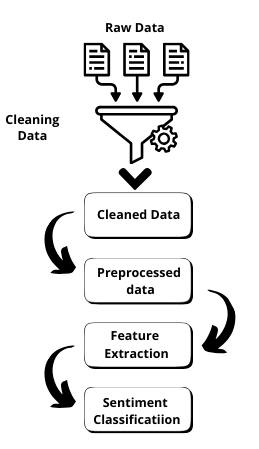
\includegraphics[width=0.2\textwidth]{archi_ml.png}
    \caption{Proposed Architecture for Darija Sentiment Analysis: Pipeline showing data preprocessing, feature extraction, and classification stages for analyzing Moroccan dialect text}
    \label{fig:architecture}
\end{figure}

\section{Methodology}
This chapter details the methodology employed for classifying sentence sentiment. It describes the text models, dataset, and classifiers used, along with the preprocessing and normalization techniques designed to handle the informal nature of dialectal Arabic, particularly Moroccan Darija. The evaluation metrics used to assess sentiment classification performance are also presented. The methodology can be summarized as follows: a description of the dataset used in this work; the application of various preprocessing steps, including normalization, noise removal, and conversion of emoticons to text, to enhance classification performance; an explanation of the techniques used for text representation; and finally, the classification of Moroccan dialect text using machine learning, deep learning, and fine-tuned pretrained model classifiers, followed by a comparison of the results.\\
To demonstrate the functionality of the sentiment analysis model, we deployed it in a web application, which can be accessed at \cite{weblink}. The app allows users to input text or Youtube video Link and receive real-time sentiment predictions based on the model.

\subsection{Data Collection}
The data collection process involved multiple sources to ensure diversity in the dataset:\\

\textbf{Existing Datasets:} Five different pre-existing datasets were leveraged:  \\
\\- Dataset 1 \cite{data1} \textbf{MAC (Moroccan Arabic Corpus)}: – A free and large corpus consisting of 18,000 manually labeled tweets, MAC is the first and largest Moroccan Arabic corpus for sentiment analysis, praised for its size, and accessibility to the research community. It provides a benchmark for future work, including polarity classification and language identification.  
\\- Dataset 2 \cite{data2} \textbf{OMCD (Offensive Moroccan Comments Dataset)}: – This dataset focuses on detecting offensive content, such as verbal attacks and hate speech, in Moroccan Arabic on social media. It is the first of its kind for the Moroccan dialect, offering annotated data for detecting offensive language in Dialectal Arabic (DA).
\\- Dataset 3 \cite{data3} \textbf{Moroccan Darija Offensive Language Detection Dataset}: – This dataset contains 20,402 Moroccan Darija sentences, labeled as either offensive or non-offensive, and gathered from Twitter and YouTube comments. 
\\- Dataset 4 \cite{data4} \textbf{ElecMorocco2016}: – A sentiment analysis dataset containing 10,254 Arabic Facebook comments related to the 2016 Moroccan elections. The comments are written in both Standard Arabic and Moroccan Dialect (Darija), offering insights into political sentiments during the election period.  
\\- Dataset 5 \cite{data5} \textbf{Covid-19 Sentiment Analysis Dataset}: – A dataset containing Facebook comments during the Covid-19 pandemic, focused on sentiment analysis and public opinion during this global crisis. The dataset includes comments in both Standard Arabic and Moroccan Dialect (Darija).\\\\
\textbf{YouTube API Data Collection:} The dataset was enriched by:
    \\- Extracting comments from popular Moroccan YouTube channels.
    \\- Focusing on videos with high engagement rates.
    \\- Collecting comments from diverse topics (reactions, programs, lifestyle).\\\\
\textbf{Data Processing Steps for the collected comments:}
    \\- Preprocessing and cleaning the collected text.
    \\- Removing duplicates and irrelevant content.
   \\- Using K-means clustering for sentiment annotation, where the DarijaBERT-Arabizi pre-trained model \cite{darijabert} was used to obtain sentence embeddings. Specifically, the embeddings were extracted from the last hidden layer of the pre-trained model \cite{emb}, capturing contextual representations of the text. These embeddings were then utilized to perform clustering and identify similarities between the collected text.

    - Validation of clustering results through human review.

    \begin{figure}[h!]
    \hspace{-1cm}
    \centering
    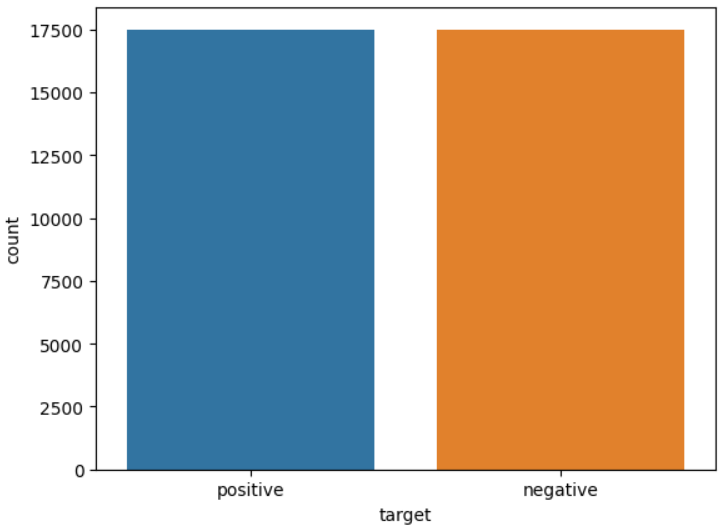
\includegraphics[width=0.5\textwidth]{data.png}
    \caption{Balanced target distribution}
    \label{fig:architecture}
    \end{figure}

    
The Production dataset used for training and evaluation is balanced, ensuring a fair representation of both positive and negative sentiments.


\subsection{Data Cleaning and Preprocessing}
Cleaning and preprocessing techniques are fundamental in Sentiment Analysis (SA) for Arabic dialectal text, particularly for the Moroccan Darija dialect. This necessity arises from the unique challenges presented by social media text, which is characterized by its informal nature and lack of standardization. The implementation addresses these challenges through a comprehensive preprocessing pipeline specifically designed for Darija text, operating at multiple levels of text normalization.

The preprocessing approach is distinguished by its specialized handling of Darija's dual-script nature (Latin and Arabic) and its complex morphological structure. The preprocessing pipeline consists of the following steps:

\begin{itemize}
    \item \textbf{Class Adaptation:} Ensuring that data across different datasets is consistent by aligning classes and removing any empty fields. This ensures that the dataset is clean and usable for further analysis.
    
    \item \textbf{Stop Words Removal:} Removal of stop words in both Arabic script and Arabizi (Latin script) representations of Darija words. This dual-script approach ensures comprehensive removal of non-informative words regardless of their writing system. The stop words lists are sourced from various reputable lexicons, including:
    \begin{itemize}
        \item Arabic Stop Words \cite{stop1} and \cite{stop2} .
        \item Moroccan stop words \cite{stop3} and  \cite{stop4} .
        \item DODa stop words (Arabizi , arabic)\cite{stop5} .
\end{itemize}

\subsubsection{Data Cleaning}
Cleaning is focused on eliminating irrelevant or noisy elements from the dataset. This step ensures that the data is free from non-informative parts, which could negatively affect the model's performance. The cleaning steps include:

\begin{itemize}
    \item \textbf{Noise Removal:} Removal of special characters, punctuation marks, numbers in both Arabic and Latin scripts, redundant or spamming alphabets, and other unwanted symbols that do not contribute to the sentiment analysis task.
    \item \textbf{Context-Aware Cleaning:} Handling modern social media elements, including:
    \begin{itemize}
        \item Emojis translation to text using a dedicated library.
        \item Removal of URLs, Emails, underscores, special tags (e.g., \&amp;, ..), and HTML tags.
        \item Removal of YouTube timestamps.
    \end{itemize}
\end{itemize}

\subsubsection{Text Preprocessing}
Preprocessing techniques prepare the text for effective analysis by transforming it into a standard format. This step includes:

\begin{itemize}
    \item \textbf{Custom Latin-to-Arabic Mapping:} A character mapping system that handles various romanized representations of Arabic phonemes for exemple :
     \begin{figure}[h!]
    \hspace{0cm}
    \centering
    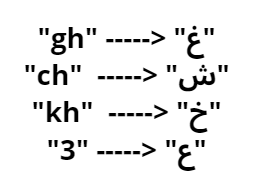
\includegraphics[width=0.3\textwidth]{traduction.png}
    \caption{Darija transliteration mapping}
    \label{fig:architecture}
\end{figure}
    
    \item \textbf{Normalization:} 
    \begin{itemize}
        \item Removal of diacritical marks (tashkeel).
        \item Elimination of elongation characters (tatweel).
        \item Standardization of various forms of hamza and alef.
        \item Removal of definite article "AL" prefix.
    \end{itemize}
 \begin{figure}[h!]
    \hspace{0cm}
    \centering
    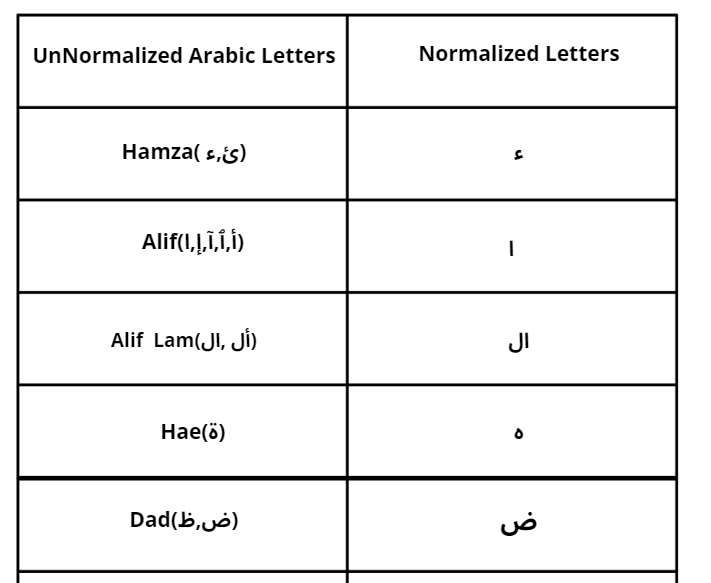
\includegraphics[width=0.5\textwidth]{norm.png}
    \caption{Normalization of  some arabic letters}
    \label{fig:architecture}
\end{figure}
    
    \item \textbf{Stemming:} Application of Arabic-specific stemming techniques using the Tashaphyne light stemmer and custom suffixes and prefixes scraped from \cite{suf1} specific to Moroccan Darija to reduce morphological variants to their base forms.

\end{itemize}

This comprehensive approach ensures that the text maintains its semantic integrity while being standardized for effective sentiment analysis, resulting in a balanced dataset with over 17,500 positive sentences and a similar number of negative sentences.

\end{itemize}


\subsection{Feature Extraction}

Feature extraction is a critical step in transforming textual data into numerical representations for analysis. Several approaches are utilized in this context, including Bag of Words, Binary Bag of Words, and Term Frequency-Inverse Document Frequency (TF-IDF).

\subsubsection{Bag of Words}
The Bag of Words (BoW) model generates a vector representation of text by counting the frequency of each word's occurrence. BoW is frequently employed in text classification and document recognition tasks due to its simplicity and effectiveness. However, this approach does not account for the importance of rare words or their distribution across the corpus.

\subsubsection{Binary Bag of Words}
The Binary Bag of Words (Binary BoW) is a variation of the BoW model, where the presence or absence of a word in a document is recorded as a binary value (1 if the word appears, 0 if it does not). This method simplifies the representation by focusing solely on the occurrence of words, ignoring their frequencies.


\subsubsection{TF-IDF}
To address the limitations of BoW, Term Frequency-Inverse Document Frequency (TF-IDF) is employed. This method assigns weights to words based on their relevance in a document and their distribution across the entire corpus. Words that appear frequently in a document but rarely in the corpus are given higher weights, enhancing their discriminative power.

\begin{figure}[h!]
    \hspace{0cm}
    \centering
    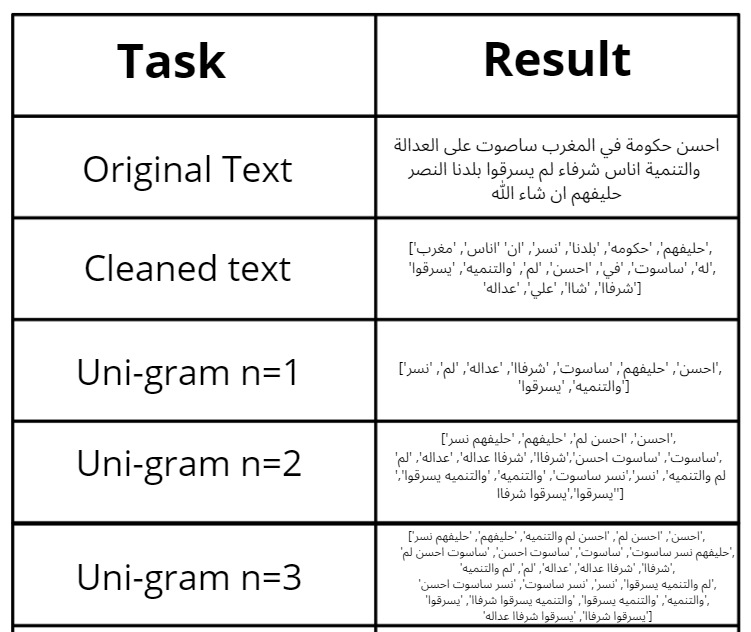
\includegraphics[width=0.5\textwidth]{text_man.png}
    \caption{Features Extraction}
    \label{fig:Features Extraction}
\end{figure}

The formulas for computing TF and IDF are as follows:

\textbf{Term Frequency (TF):}
\begin{equation}
\text{tf}_{i,j} = \frac{n_{i,j}}{\sum_k n_{k,j}}
\end{equation}

\textbf{Inverse Document Frequency (IDF):}
\begin{equation}
\text{idf}_i = \log{\frac{N}{\text{df}_i}}
\end{equation}

\textbf{TF-IDF Weight:}
\begin{equation}
w_{i,j} = \text{tf}_{i,j} \times \text{idf}_i
\end{equation}

Where:
\begin{itemize}
    \item $n_{i,j}$ is the number of occurrences of term $i$ in document $j$.
    \item $\text{df}_i$ is the number of documents containing the term $i$.
    \item $N$ is the total number of documents in the corpus.
\end{itemize}

TF measures the frequency of a term in a document, while IDF reduces the weight of common terms across the corpus. The resulting TF-IDF matrix has dimensions $(\text{documents} \times \text{vocabulary})$, capturing the importance of terms across the entire dataset.

This approach allows for effective handling of common and rare terms, ensuring robust text analysis.

 
\section{Classification Models}

Several classification algorithms were tested and tuned to perform sentiment analysis. Each model brought valuable insights, and although multiple approaches showed promising results, the Support Vector Machine (SVM) with TF-IDF and bigrams ultimately delivered the best performance. All models were carefully tuned using hyperparameter optimization techniques to ensure their best possible performance. Below, we describe the models tested and explain why the SVM model was selected.



\subsection{Machine Learning Models}

\subsubsection{Logistic Regression}
Logistic Regression is a linear model that predicts the probability of a class using a sigmoid function. It's often used for binary classification tasks due to its simplicity and interpretability. Although it performed reasonably well as a baseline model, its performance was limited by its inability to capture complex dependencies between words in the text.

\subsubsection{Multinomial Naive Bayes}
The Multinomial Naive Bayes classifier is particularly suited for text classification, where features represent word frequencies or counts. It is a probabilistic model based on Bayes' Theorem, assuming independence between features. While it performed decently, its assumption of feature independence limited its ability to model more complex relationships in the text.

\subsubsection{Decision Tree}
A Decision Tree classifier uses a tree-like structure to make predictions by recursively splitting the data based on feature values. It is easy to interpret and visualize but can be prone to overfitting, especially with high-dimensional data like text.

\subsubsection{Random Forest}
Random Forest is an ensemble learning method that combines multiple decision trees to improve prediction accuracy. It generally performs well with high-dimensional data and helps to reduce overfitting. While Random Forest performed adequately, it did not outperform the selected SVM model in terms of accuracy and efficiency for this specific problem.

\subsubsection{XGBoost}
XGBoost is a gradient boosting algorithm that iteratively corrects the errors made by previous models, often leading to very high accuracy. However, it requires significant computational resources and hyperparameter tuning, making it less efficient compared to the selected SVM model.

\subsection{Deep Learning Models}
\subsubsection{Convolutional Neural Networks (CNNs)}
CNN is effective at capturing local patterns and dependencies in the text, especially in shorter sequences. However, CNNs were not able to outperform traditional machine learning models for this task, likely due to the relatively small size and structure of the dataset.

\subsubsection{Recurrent Neural Networks (RNNs)}
RNN is designed for sequential data, maintaining hidden states that capture contextual dependencies between words. While they were able to capture more complex relationships in the text, they required more computational power and did not significantly improve upon the results of simpler models for this specific sentiment analysis task.

\subsection{Pre-trained Large Language Models}

In recent years, pre-trained large language models (LLMs) have demonstrated significant potential in various natural language processing (NLP) tasks, including sentiment analysis and text classification. These models, particularly those based on the transformer architecture, have been fine-tuned for specific languages and dialects to enhance their performance on specialized tasks. For Moroccan Darija, which presents unique challenges such as informal language, code-switching, and a lack of standardization, several pre-trained models have been explored to address these complexities.

While models like BERT have shown success across multiple languages, applying them to Darija requires careful adaptation to its unique structure. From my experience, fine-tuning these models for Darija has proven to be particularly challenging due to the informal and non-standardized nature of the dialect. Additionally, the need for substantial computational resources and high-quality labeled data has been a significant barrier. The process of fine-tuning for Darija is further complicated by code-switching between Arabic, French, and other languages, which is common in social media texts. Pre-trained models specifically designed for Moroccan Arabic or Arabizi text offer a more tailored approach to capture these linguistic features. Notable examples include DarijaBERT-Arabizi \cite{darijabert}, DarijaBERT \cite{darijabert}, and MorrBERT \cite{morrbert}, each showing varying degrees of success in processing Moroccan Darija text. However, despite promising results, fine-tuning these models has not consistently led to superior performance compared to traditional machine learning models.

\begin{figure}[H]
    \centering
    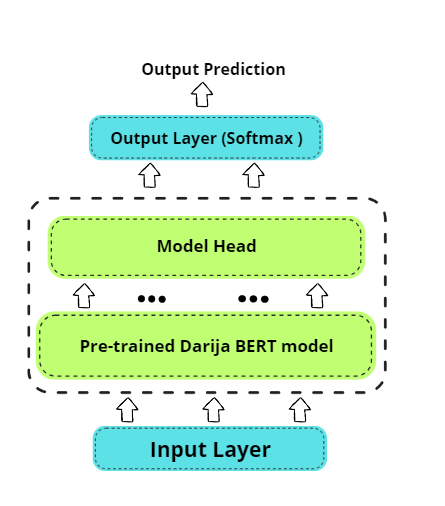
\includegraphics[width=0.4\textwidth]{bert.png}
    \caption{BERT Architecture}
    \label{fig:BERT ARCHI}
\end{figure}

\subsection{Selected Model: Support Vector Machine (SVM) with TF-IDF Vectorizer}

The Support Vector Machine (SVM) model with TF-IDF and bigrams emerged as the best-performing model for this sentiment analysis task. This model was chosen due to its excellent balance between accuracy and computational efficiency. The following parameters were used for the SVM model after tuning the hyperparameters using GridSearch:

\begin{itemize}
    \item \( C = 1.0 \): The regularization parameter, which controls the trade-off between achieving a low error on the training data and minimizing the margin.
    \item \texttt{kernel='rbf'}: The radial basis function kernel, which allows the model to handle non-linear decision boundaries effectively.
    \item \texttt{gamma='scale'}: A kernel coefficient value that adapts to the data, ensuring optimal performance.
\end{itemize}

\subsubsection{Formal Description}
The SVM algorithm aims to find the optimal hyperplane that maximizes the margin between the two classes. The optimization problem is formulated as:

\[
\min_{w,b,\xi} \frac{1}{2} \|w\|^2 + C \sum_{i=1}^{n} \xi_i
\]

subject to the constraints:

\[
y_i (w^T x_i + b) \geq 1 - \xi_i, \quad \xi_i \geq 0, \quad \forall i = 1, \dots, n
\]

where \( w \) is the weight vector, \( b \) is the bias, \( \xi_i \) are the slack variables, and \( C \) is the regularization parameter.

The hinge loss function, which SVM uses during training, is defined as:

\[
L(y_i, f(x_i)) = \max(0, 1 - y_i f(x_i)),
\]

where \( f(x_i) = w^T x_i + b \) is the decision function. This loss penalizes misclassified points and those within the margin, ensuring that the model not only classifies points correctly but also maintains a margin around the hyperplane.

The TF-IDF vectorizer was used to convert text data into numerical features, and bigrams were incorporated to capture contextual relationships between adjacent words. The use of bigrams allowed the model to better capture the nuances of sentiment in text, especially for informal dialects like Darija. TF-IDF weighted the importance of words based on their frequency and relevance, improving the model's ability to distinguish between relevant features and noise.

\subsubsection{Why SVM with TF-IDF and Bigrams?}
SVM with TF-IDF and bigrams provided several advantages over other models:
\begin{itemize}
    \item \textbf{Efficiency:} SVM is computationally efficient compared to deep learning models, particularly when the dataset is not very large.
    \item \textbf{Effectiveness with Text Data:} The combination of TF-IDF and bigrams allowed the model to capture important word pair relationships that are crucial for understanding sentiment in informal text.
    \item \textbf{Interpretability:} SVM offers interpretability, making it easier to understand the decisions made by the model.
    \item \textbf{Scalability:} SVM with TF-IDF and bigrams can scale well to larger datasets with minimal loss in performance.
\end{itemize}

While other models were tested, SVM with TF-IDF and bigrams outperformed them in terms of both accuracy and efficiency, making it the most suitable choice for this sentiment analysis task.
\section{Evaluation}

The evaluation of the model was conducted using standard classification metrics to assess its performance comprehensively. The metrics used are as follows:

\begin{itemize}
    \item \textbf{Accuracy:} Measures the proportion of correct predictions (both true positives and true negatives) out of the total number of predictions. In this case, the accuracy is 0.77, indicating that 77\% of predictions were correct.
    
    \item \textbf{Precision:} Precision is the proportion of positive predictions that are actually correct. It is particularly important in scenarios where the cost of false positives is high.
    \[
    \text{Precision} = \frac{TP}{TP + FP}
    \]
    where $TP$ (True Positives) represents the correctly identified positive cases, and $FP$ (False Positives) represents the cases incorrectly identified as positive.
    
    \item \textbf{Recall:} Also known as sensitivity, recall measures the proportion of actual positives that are correctly identified. It is crucial when the cost of false negatives is high.
    \[
    \text{Recall} = \frac{TP}{TP + FN}
    \]
    where $FN$ (False Negatives) represents the positive cases incorrectly identified as negative.
    
    \item \textbf{F1-Score:} The F1-score is the harmonic mean of precision and recall, providing a balance between them. It is particularly useful when there is an imbalance between classes.
    \[
    F1 = 2 \cdot \frac{\text{Precision} \cdot \text{Recall}}{\text{Precision} + \text{Recall}}
    \]
\end{itemize}

The results for each class are as follows:
\begin{itemize}
    \item \textbf{Positive class:} Precision = 0.76, Recall = 0.79, F1-Score = 0.78, Support = 3443.
    \item \textbf{Negative class:} Precision = 0.77, Recall = 0.74, F1-Score = 0.76, Support = 3322.
\end{itemize}

\textbf{Confusion Matrix:}
The confusion matrix provides a detailed breakdown of the model's performance. It is structured as follows:
\begin{itemize}
    \item \textbf{True Positives (TP):} Correctly identified positive cases (2728).
    \item \textbf{False Positives (FP):} Cases incorrectly identified as positive (715).
    \item \textbf{True Negatives (TN):} Correctly identified negative cases (2458).
    \item \textbf{False Negatives (FN):} Cases incorrectly identified as negative (864).
\end{itemize}

\begin{figure}[H]
    \centering
    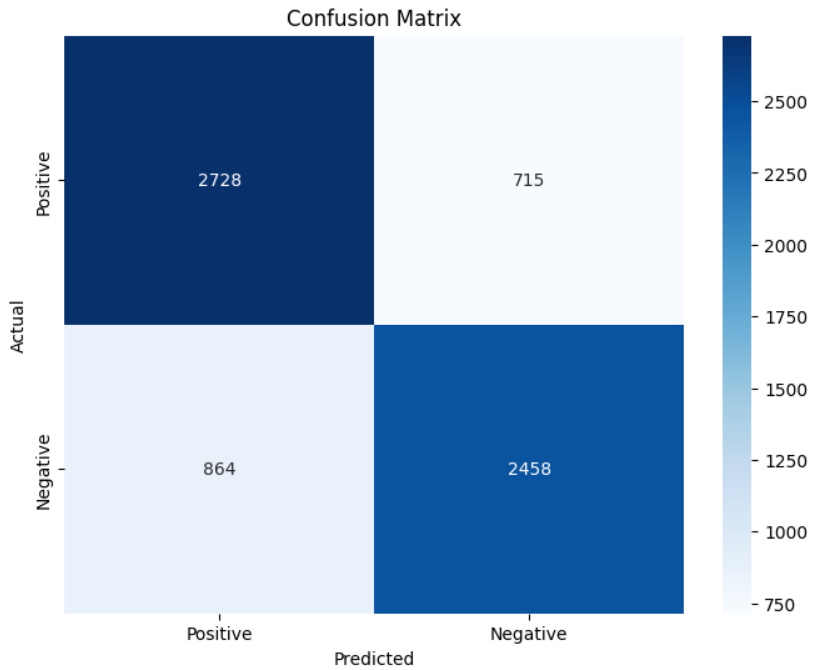
\includegraphics[width=0.5\textwidth]{svm_eval.png}
    \caption{Confusion Matrix for the SVM Model}
    \label{fig:confusion_matrix}
\end{figure}
\begin{figure}[H]
    \centering
    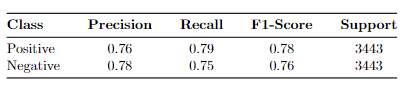
\includegraphics[width=0.5\textwidth]{metrics.png}
    \caption{Classification Performance Evaluation Metrics}
    \label{fig:ClassificationMetrics}
\end{figure}

The confusion matrix and table of Performance (Figure \ref{fig:confusion_matrix}, \ref{fig:ClassificationMetrics} ) highlights how well the model performed on each class and provides insights into areas where the model can be improved.


\begin{figure}[H]
    \centering
    
\includegraphics[width=0.5\textwidth]{cloud_pos.png}
    \caption{Positive class word occurrence}
    \label{fig:positive words}
\end{figure}
%-------------------------------------------------
\section{Model Performance and Benchmark}
\subsection{Testing of Models Results }

The performance of various ML classifiers using different feature extraction techniques is summarized in Figure~\ref{fig:ml_results}. Similarly, the accuracy of deep learning models and fine-tuned pre-trained models is presented in Figure~\ref{fig:dl_bert_results}.

\begin{figure*}[t] % Full-width figure
    \centering
    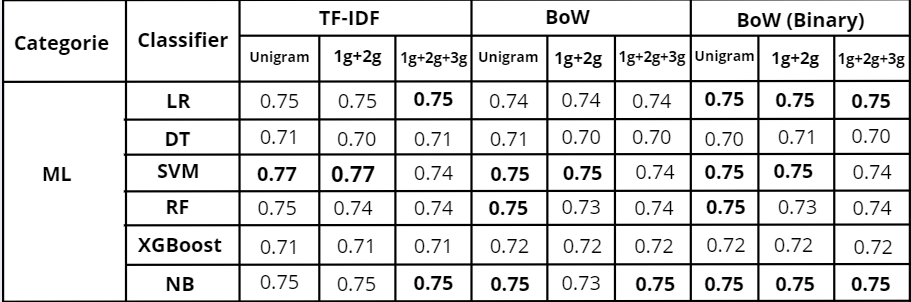
\includegraphics[width=\textwidth]{dl_bert.png}
    \caption{Accuracy of ML classifiers with different feature extraction methods (TF-IDF, BoW, and BoW Binary).}
    \label{fig:ml_results}
\end{figure*}

\begin{figure}[H]
    \centering
    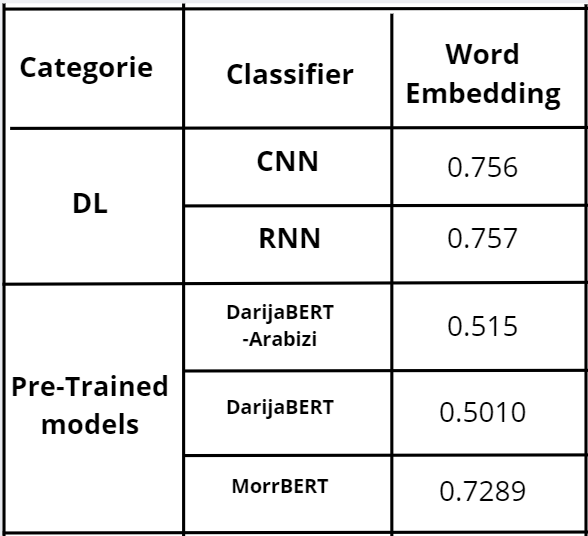
\includegraphics[width=0.6\linewidth]{ml.png}
    \caption{Accuracy comparison of DL models and fine-tuned pre-trained models.}
    \label{fig:dl_bert_results}
\end{figure}

\subsection{Benchmark Comparison}

The table below compares the performance metrics of the models based on accuracy, F1-score, precision, and recall.

\begin{table}[H]
\captionsetup{type=figure} 
\centering
\scriptsize
\begin{tabular}{lcccc}
\hline
\textbf{Model} & \textbf{Precision} & \textbf{Recall} & \textbf{F1-Score} & \textbf{Accuracy} \\ \hline
SVM            & 0.77              & 0.77            & 0.77              & 0.77             \\ 
Hamza Model    & 0.74              & 0.74            & 0.74              & 0.74             \\ \hline
\end{tabular}
\caption{Performance Comparison of Models}
\label{fig:benchmark}
\end{table}







\section{Limitations of the Approach}
Despite the growing presence of Darija in written form across various platforms, processing it poses several unique challenges. These difficulties arise from the specific characteristics of the language, which complicate its handling in natural language processing (NLP) tasks. Some of the key challenges include:



\begin{itemize}
    \item \textbf{Lack of Standardization:} Darija lacks a standardized orthography, leading to variations in spelling and writing conventions. For example:
    \begin{itemize}
        \item The word "Good" can be written as "mzian," "mezyan," or "meziane."
        \item "What" can be written as "chno," "chnou," "chnowa," or "cheni."
    \end{itemize}

    \item \textbf{Code-Mixing:} Darija frequently mixes with French, English, and Modern Standard Arabic (MSA), creating code-switched text that complicates language processing. For example:
    \begin{itemize}
        \item "khoya had weekend ghadi nmchiw ndiro shopping" (My brother, we’ll go shopping this weekend)
        \item "C'est bon, fhemtek" (It's good, I understand)
    \end{itemize}

    \item \textbf{Informal Nature:} The informality of Darija, especially on social media, complicates the application of traditional NLP techniques. For example:
    \begin{itemize}
        \item Using numbers as letters: "3ayane" instead of "aayane" (tired)
        \item Elongating letters for emphasis: "mziaaaaaaan" instead of "mzian" (good)
        \item Using abbreviations: "wlh" instead of "wallah" (I swear)
    \end{itemize}
\end{itemize}

These challenges are not limited to sentiment analysis but affect a wide range of NLP applications, including machine translation, information retrieval, and text summarization.

\section{Conclusion}

This study investigated sentiment analysis for Moroccan Darija, addressing the unique linguistic challenges of this non-standardized Arabic dialect. Contributing to the broader field of NLP in informal linguistic contexts, we demonstrated the effectiveness of both traditional and deep learning approaches. Using a semi-supervised labeling approach leveraging k-means clustering on embedding vectors for initial labeling followed by meticulous manual correction to have a valuable labeled resource. Experiments showed that traditional machine learning models (Multinomial Naive Bayes, Logistic Regression, XGBoost, SVM) and deep learning models (CNN and RNN) achieved promising results after hyperparameter optimization. However, fine-tuned BERT-based models (like DarijaBERT) did not yield the expected performance gains, suggesting the need for further research into optimal fine-tuning, architectural modifications, alternative pre-training, larger datasets, or alternative architectures better suited to Darija. We acknowledge limitations including potential data biases and computational demands. Despite these, this research offers valuable insights into Darija sentiment analysis and underscores the importance of addressing linguistic diversity in real-world NLP applications. \\
Looking ahead, we plan to further enhance our sentiment analysis model by integrating more advanced deep learning techniques, such as LSTM, and experimenting with fine-tuning strategies to improve performance. We will also explore alternative feature extraction methods that could lead to better accuracy. Additionally, we aim to broaden our dataset by including a wider variety of Moroccan Arabic sources and incorporating additional topics to enhance the model's performance across a broader range of subjects.


\printbibliography
\end{document}